
\section{The Motion Capture Module}
\label{sec:the_motion_capture_model}

The Motion Capture Module is responsible for integration with the Qualisys Motion Capture System. It takes measurements from the camera system, and integrates them in the SML World.

\subsection{Module Structure}

A simple diagram of the Module is shown in \ref{fig:motion_capture_module_diagram}. The Motion Capture Module is part of the SML World, running on its own thread, and having access to the Bodies Dictionary, thus being able to interact with and changing them. The Motion Capture Module, uses the QualisysComms class in order to establish a communication link with the Qualisys Software being hosted at the Qualisys Computer located in the SML.

\begin{figure}[h!]
  \centering
    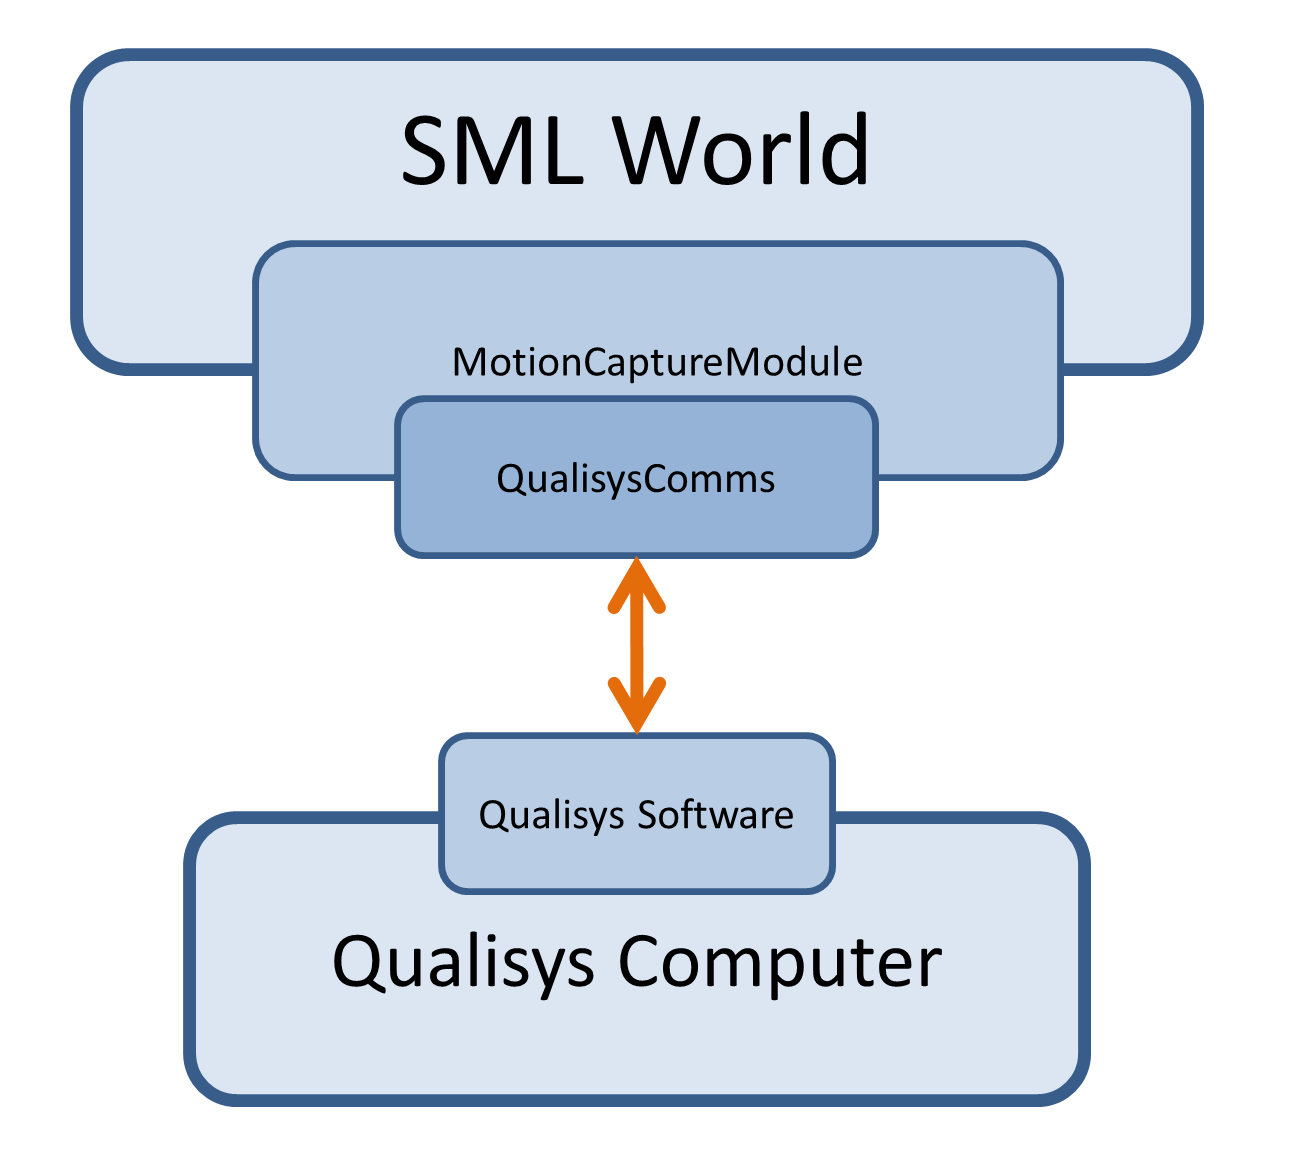
\includegraphics[width=0.8\textwidth]{motion_capture_module_diagram}
    \caption{The Motion Capture Module structure \label{fig:motion_capture_module_diagram} }
\end{figure}

The Python code developed for communications with the Qualisys Motion Capture System was originally developed by Matteo Vanin, and can be found in \texttt{QualisysComms.py}. 

\subsection{Constructor}

The Motion Capture Module constructor takes as argument the instance of the SML World, so that it can have access to the Bodies Dictionary and interact with it. As optional parameters one has:

\begin{description}
\item[\texttt{qualisys\_host}] The IP of the Qualisys Computer, where the Motion Capture software is running. If not provided, the argument will default to \texttt{'sml-qualisys.ddns.net'}
\item[\texttt{qualisys\_port}] The port where the Motion Capture software is running its connection server. If not provided, the argument will default to \texttt{'22224'}, the default server port of the software.
\item[\texttt{desired\_rate}] The rate at which we want the tracked bodies to be refreshed.
\end{description}

The IP address of the Qualisys computer can be found by running the simple \texttt{ipconfig} command on the terminal. However, the Qualisys computer is running an application which associates it's IP to the \texttt{'sml-qualisys.ddns.net'} name. Meaning that if one tries to resolve this address name, one will end up getting the current IP of the Qualisys computer. The software used to achieve this functionality is NO-IP \cite{no-ip}.

The constructor also launches a new thread which will be running while the SML World is active. This thread will loop at a rate \texttt{desired\_rate}, and will at every iteration update the real vehicles (\textit{i.e.}, vehicles/bodies with a physical correspondence in the lab), so that they correspond to the most current pose estimate provided by the Qualisys Motion Capture system.

\subsection{From the Lab to the SML World}

The Motion Capture System, provided the users with pose estimates (6 DOF) for objects being tracked. These estimates are polled by the Motion Capture Module, which will then process them. We can distinguish the Vehicles/Bodies in the SML World, into two broad categories, simulated and real. The simulated ones, are completely virtual, and the real ones are based on real vehicles/bodies captured from the Qualisys System, and then added to the virtual environment. As an implementation detail, real vehicles are attributed a positive id (unique identifier), which corresponds to the id they posses in the Qualisys System. And simulated vehicles are assigned negative ids.

Once the Motion Capture System gets the poses from the tracked bodies, it will first check if the current Bodies List of the SML World contains a Vehicle with the same id, in case it does not, it will create a new Body and add it to the SML World bodies list. To know the specific class created, the user should check the implementation.

In case the body already exists, the Module will simply update its state, in order to correspond to the current pose estimate. Since we are dealing with $1:32$ scaled vehicles (we are using the mini trucks), and since the SML World is a simulation of a real scale world, we need to multiply the state position estimate by a factor of 32, and only then set this as the new position of the vehicle.